\section{Question 1: Workload structure and capacity pressure}
\label{sec:r1q1}
The supplied trace has 224,112 jobs on 4,278 nodes, with 10,412 GPUs and 632,636 vCPUs across six GPU models. For job $j$, $a_j$ is release time, $p_j$ duration, $W_j$ workers, and $(g_j,c_j)$ the per-worker GPU and vCPU requests. Submitted GPU work is $H_j=W_jg_jp_j$; it is a request-based quantity, not measured device utilization. The six isolated pools are summarized in Table~\ref{tab:r1pools}. The exact input hashes and the serialization comparison are in the provenance record, so the claims below use the formal-run CSV.

\begin{table}[H]\centering\caption{Six pools under the SPT-HOL full-cluster evidence. Waiting uses complete drain; allocation and completion use $[0,H)$ with $H=7,776,000$ s.}\label{tab:r1pools}\begin{tabular}{lrrrrrr}
\toprule
Pool & Jobs & GPUs & Mean wait (h) & Median/P99 (h) & GPU/CPU alloc. & $90$d done\\
\midrule
A10 &111,284&2,494&32.906&0.023/1542.181&99.922\%/17.927\%&107,002\\
A100-SXM4-80GB&80,877&3,456&0.000&0.000/0.000&62.755\%/42.032\%&80,101\\
GPU-series-1&9,643&1,558&0.434&0.000/14.492&60.779\%/34.787\%&8,213\\
GPU-series-2&13,633&976&0.016&0.000/0.045&56.931\%/37.424\%&13,606\\
H800&4,716&1,752&0.016&0.000/0.000&55.816\%/52.193\%&4,705\\
A800-SXM4-80GB&3,959&176&0.115&0.000/4.390&57.311\%/49.493\%&3,943\\
\bottomrule
\end{tabular}\end{table}

\begin{figure}[H]\centering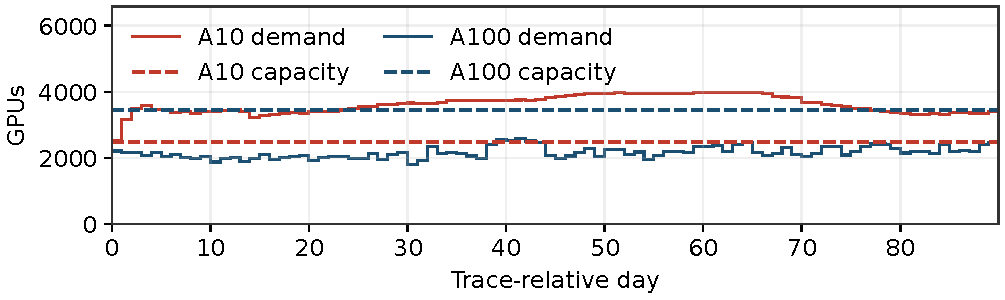
\includegraphics[width=\linewidth]{r1_figures/fig1_demand.pdf}\caption{Exact daily-bin overlap of the immediate-start counterfactual and physical GPU capacity. This is demand/capacity, not simulated allocation. The A10 mean is 3,614.54 GPUs against 2,494 capacity and its peak is 4,103; A100 demand stays below its 3,456-GPU capacity.}\label{fig:r1demand}\end{figure}

The workload is concentrated: GPU-work Gini is 0.9522, the top 1\% (2,241 jobs) contributes 43.30\%, and the top 5\% (11,205 jobs) contributes 87.68\%. Median duration is 1,330 s, the 95th percentile is 309.09 h, and the maximum is about 184 days. There are 3,512 jobs at trace time zero; without a calendar origin, their position is reported as a trace-origin batch rather than a weekday effect. The exposure-corrected relative 24-hour profile peaks at phase hour 16 and is lowest at hour 4 (ratio 2.29); this is a relative phase diagnostic, not a timezone claim.

The shape is also strongly single-worker: 90.95\% of jobs use one worker, 78.42\% use one GPU per worker, and the means are 1.539 workers and 2.003 GPUs per worker. Daily arrivals are nonstationary at the trace scale: the first day contains 8,509 jobs, day 1 contains 5,525, and the minimum is 965 jobs on day 63. These counts describe the observed window and do not identify a calendar effect or a particular arrival process.

\begin{figure}[H]\centering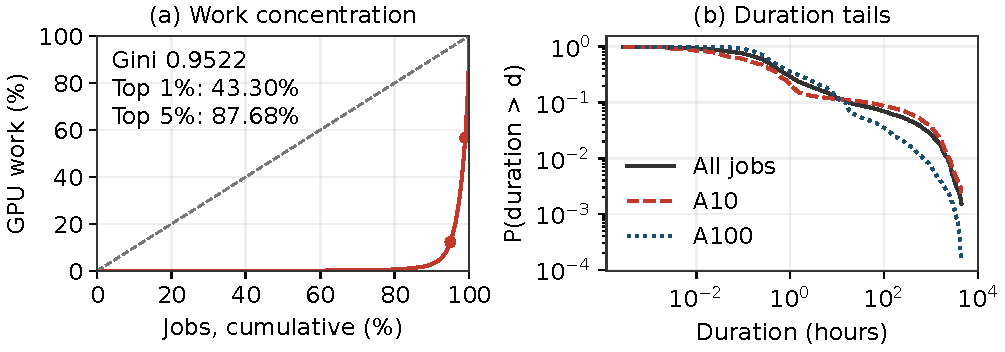
\includegraphics[width=\linewidth]{r1_figures/fig1_data_patterns.pdf}\caption{Two high-information views of the formal data: cumulative GPU-work concentration and strict duration tails.}\label{fig:r1patterns}\end{figure}

For model $m$, with exact Q1 observation window $T=7,775,878$ s, the lifetime-work ratios are
\begin{equation}
\rho_m^{GPU}=\frac{\sum_{j\in\mathcal J_m}W_jg_jp_j}{T\sum_{i\in\mathcal I_m}G_i},\qquad
\rho_m^{CPU}=\frac{\sum_{j\in\mathcal J_m}W_jc_jp_j}{T\sum_{i\in\mathcal I_m}C_i}.
\end{equation}
A10 has $\rho^{GPU}=2.064$ (Table~\ref{tab:r1pools} reports the corresponding pool work context), while GPU-series-1 has a shape mismatch: 2,478 jobs (25.70\% of that pool, 78.07\% of its work) exceed the 24-vCPU/GPU ratio of its 8-GPU, 192-vCPU nodes. The 24-, 48-, 128- and 192-vCPU/GPU configurations contain 77, 10, 1 and 901 nodes respectively. This motivates node-level gang checks; it does not identify a unique bottleneck policy.

Two lower bounds are retained with their objectives. The GPU-work weighted A10 waiting bound is 560.521 h and weights job $j$ by $H_j$. The Q2 job-count bound is 22.3179305700 h and weights every job equally. Neither is an allocation rate, an OPT value, or a guarantee after substitution changes capacity or duration.
